RGG allows you to provide paths to AssyGen and CoreGen (provided by MeshKit\footnote{See \url{http://trac.mcs.anl.gov/projects/fathom/wiki/MeshKit}.}) and Cubit\footnote{See \url{https://cubit.sandia.gov/}.} executables to facillitate the production of meshes for simulation.

\section{Add Paths to Preferences}

In order for RGG to mesh an INP file, we'll first need to provide it the paths to the AssyGen, CoreGen, and Cubit executables.

Access the \ui{system preferences window} by clicking on the \ui{edit menu} of the \ui{toolbar} on Linux and Windows.  On Mac, click on the \ui{preferences item} of the \ui{RGG Nuclear menu}.

\begin{figure}[H]
	\begin{center}
		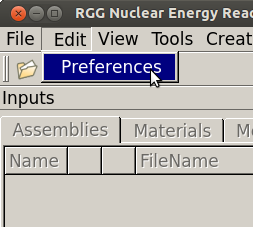
\includegraphics[width=0.5\linewidth]{Images/mesh-1.png}
		\caption{Opening RGG preferences.}
		\label{fig:Mesh1}
	\end{center}
\end{figure}

This brings up the \ui{system preferences window}.  The \ui{system preferences window} has a section for each of the three executables.  To add one, click the \ui{browse button} in the section that corresponds to the desired executable.  Locate the executable and click the \ui{open button} to get back to the system preferences window.

\begin{figure}[H]
	\begin{center}
		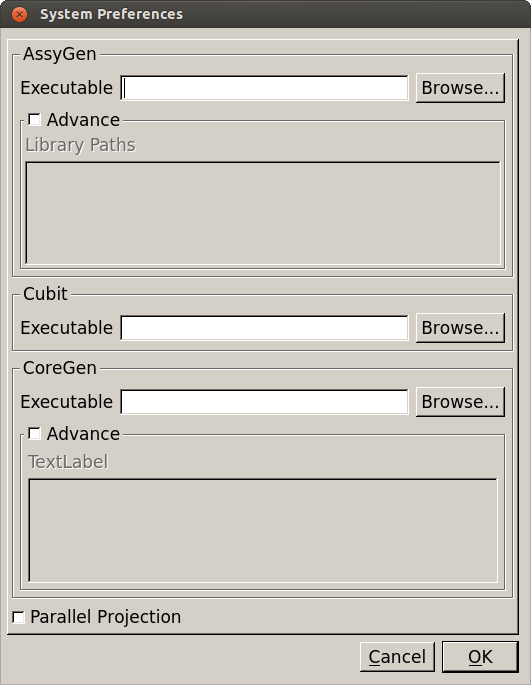
\includegraphics[width=0.5\linewidth]{Images/mesh-2.png}
		\caption{The preferences window.}
		\label{fig:Mesh2}
	\end{center}
\end{figure}

Note the \ui{advance checkbox} in the AssyGen and CoreGen sections.  If either of these executables require shared libraries in non-standard locations, you can click this checkbox to activate the \ui{library paths text box}.  You can specify directories where the shared libraries are, with each line being another location.